\clearpage
\Question{Tries}

Consider the following ternary search trie (TST):
\begin{center}
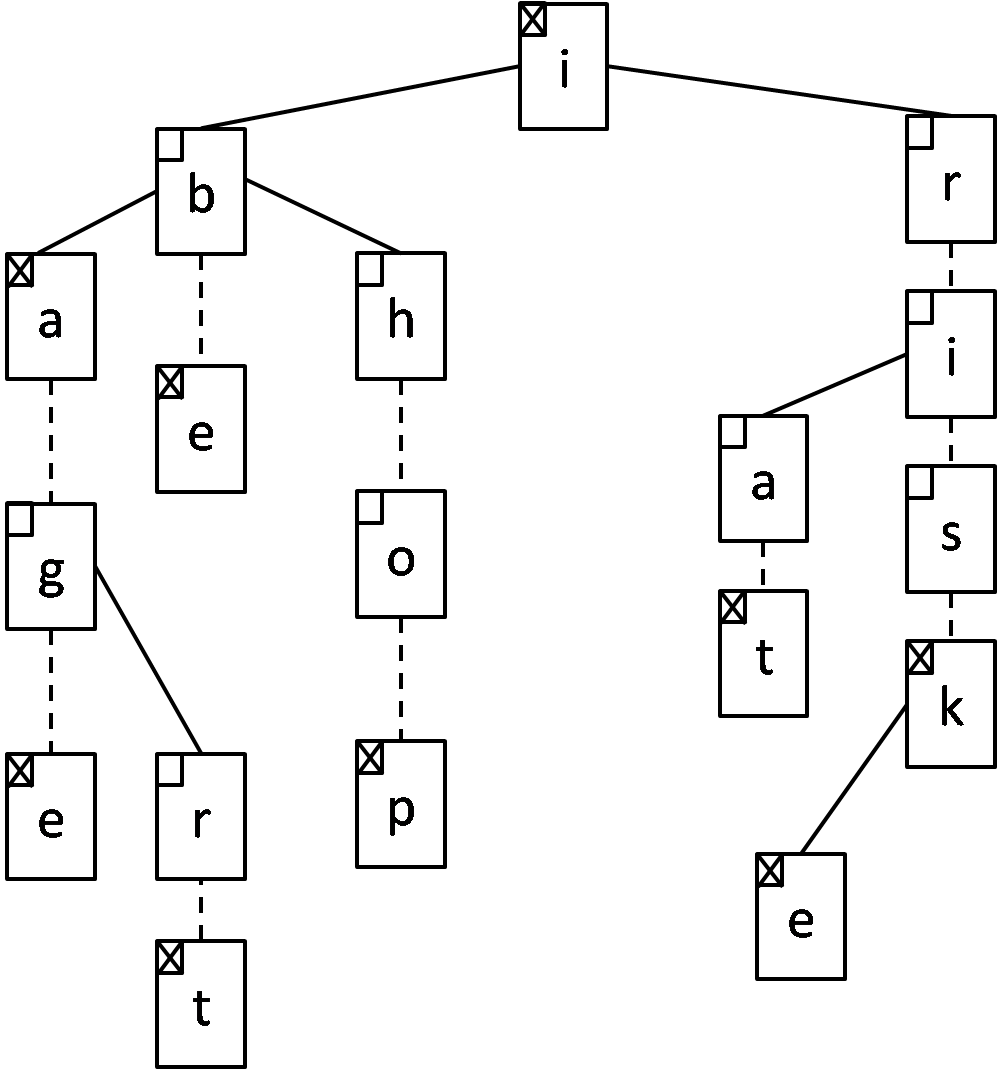
\includegraphics[width=.6\textwidth]{\img/tst3.png}
\end{center}

The dotted lines connect a node to its middle child, and solid lines
connect a node to its left and right children.  An \emph{X} in the top
left indicates that this node ends a valid word.

\begin{parts}

\part[2]\TAGS{trie}
List all of the valid words stored in the TST above, in alphabetical order.
\begin{framed}
\ifprintanswers{\color{\answerColor}
  A, AGE, ART, BE, HOP, I, RAT, RISE, RISK
}\else~\vspace{1.0in}\fi
\end{framed}

\RUBRIC
Part (a)
TAGS: trie

Gradescope rubric:  TODO

Commentary:
  A, AGE, ART, BE, HOP, I, RAT, RISE, RISK
  Half a point penalty if not alphabetical order
  Half point penalty for each missing/incorrect word
  Minimum of 0
ENDRUBRIC

\newpage
\part[1]\TAGS{trie}
Add the words
\lstinline'me',
\lstinline'rake',
\lstinline'hope',
\lstinline'hot',
\lstinline'top', and
\lstinline'act'
to the TST given on the previous page, one at a time, in the order
given.  DO not worry about rebalancing
\begin{framed}
\begin{lstlisting}[basicstyle=\basicstyle\color{\answerColor}]
           ----------i*-------
          /                   \
     ----b--         --------- r--
    /    |  \       /          |  \
   a*    e*  h     M       ----i   T
   |         |     |      /    |   |
  -g--       o     E*    a     s   O
 / |  \      |           |     |   |
C  e*  r     p--       --t*  --k*  P*
|      |     |  \     /     /
T*     t*    E*  T*  K      e*
                     |
                     E*
\end{lstlisting}
\else~\vspace{8.0in}\fi
\end{framed}

\RUBRIC
Part (b)
TAGS: trie

Gradescope rubric:  TODO

Commentary:
  - Half point per missed or incorrect insertion until they hit 0
      - CT to the left of "e"
      - E below "hop"
      - T to the right of "hop"
      - ME to the left of "r"
      - KE to the left of "rat"
      - TOP to the right of "r"
  - Max 2 half-point penalties for screwed up Xes

(original TST in lowercase, additions in uppercase)
           ----------i*-------
          /                   \
     ----b--         --------- r--
    /    |  \       /          |  \
   a*    e*  h     M       ----i   T
   |         |     |      /    |   |
  -g--       o     E*    a     s   O
 / |  \      |           |     |   |
C  e*  r     p--       --t*  --k*  P*
|      |     |  \     /     /
T*     t*    E*  T*  K      e*
                     |
                     E*
ENDRUBRIC

\newpage
\part[5]\TAGS{correctness, trie}
Write the function \lstinline'trie_height' which returns the string
length of the longest word in the trie. For example, a trie containing
the strings \lstinline'"hi"', \lstinline'"hello"', and
\lstinline'"thanks"' has a height of 6. For full credit, the helper
function \lstinline'tnode_height' must be \emph{recursive}.

\begin{framed}
\begin{lstlisting}[belowskip=0pt]
int tnode_height(tnode* T) {
\end{lstlisting}
\ifprintanswers
\begin{lstlisting}[basicstyle=\basicstyle\color{\answerColor}]
  if (T == NULL) return 0;

  int lh = tnode_height(T->left);
  int mh = tnode_height(T->middle);
  int rh = tnode_heigth(T->right);

  return max(lh, mh+1, rh);
\end{lstlisting}
\else~\vspace{4.5in}\fi
\begin{lstlisting}[aboveskip=0pt]
}

int trie_height(trie TR) {

  return tnode_height([*\uanswer{20em}{tnode\_height(TR->root)}*]);
}
\end{lstlisting}
\end{framed}
\RUBRIC
Part (c)
TAGS: correctness, trie

Gradescope rubric:  TODO

Commentary:
  tnode_height
      +1 for correct base case
      +1 for getting heights of subtrees
      +1 for correct return value max(lh,mh+1,rh)

  trie_height
      +1 for TR->root in blank

Solution:
int tnode_height(tnode* T) {
  if (T == NULL) return 0;

  int lh = tnode_height(T->left);
  int mh = tnode_height(T->middle);
  int rh = tnode_heigth(T->right);

  return max(lh, mh+1, rh);
}

int trie_height(trie TR) {
  return tnode_height(TR->root);
}
ENDRUBRIC


\end{parts}
